\documentclass[a4paper]{tufte-book}

\title{JSXGraph\thanks{Thanks to \ldots for his inspiration.}}
\author[The JSXGraph Developers]{The JSXGraph\ Developers}
\publisher{University of Bayreuth}




%%%%%%%%%%%%%%%%%%%%%%%%%%%%%%%%%%%%%%%%%%%%%%%%%%%%%%%%%%%%%%%%%%%%%%%%%%%%%%%%%%%
\usepackage{lipsum}
\usepackage{booktabs}
\usepackage{graphicx}
\setkeys{Gin}{width=\linewidth,totalheight=\textheight,keepaspectratio}
\graphicspath{{graphics/}}
%%
% If they're installed, use Bergamo and Chantilly from www.fontsite.com.
% They're clones of Bembo and Gill Sans, respectively.
\IfFileExists{bergamo.sty}{\usepackage[osf]{bergamo}}{}% Bembo
\IfFileExists{chantill.sty}{\usepackage{chantill}}{}% Gill Sans

\usepackage{microtype}

%%
% Just some sample text
\usepackage{lipsum}

%%
% For nicely typeset tabular material
\usepackage{booktabs}

%%
% For graphics / images
\usepackage{graphicx}
\setkeys{Gin}{width=\linewidth,totalheight=\textheight,keepaspectratio}
\graphicspath{{graphics/}}

% The fancyvrb package lets us customize the formatting of lstlisting
% environments.  We use a slightly smaller font.
\usepackage{fancyvrb}
\fvset{fontsize=\normalsize}

%%
% Prints argument within hanging parentheses (i.e., parentheses that take
% up no horizontal space).  Useful in tabular environments.
\newcommand{\hangp}[1]{\makebox[0pt][r]{(}#1\makebox[0pt][l]{)}}

%%
% Prints an asterisk that takes up no horizontal space.
% Useful in tabular environments.
\newcommand{\hangstar}{\makebox[0pt][l]{*}}

%%
% Prints a trailing space in a smart way.
\usepackage{xspace}

%%
% Some shortcuts for Tufte's book titles.  The lowercase commands will
% produce the initials of the book title in italics.  The all-caps commands
% will print out the full title of the book in italics.
\newcommand{\vdqi}{\textit{VDQI}\xspace}
\newcommand{\ei}{\textit{EI}\xspace}
\newcommand{\ve}{\textit{VE}\xspace}
\newcommand{\be}{\textit{BE}\xspace}
\newcommand{\VDQI}{\textit{The Visual Display of Quantitative Information}\xspace}
\newcommand{\EI}{\textit{Envisioning Information}\xspace}
\newcommand{\VE}{\textit{Visual Explanations}\xspace}
\newcommand{\BE}{\textit{Beautiful Evidence}\xspace}

\newcommand{\TL}{Tufte-\LaTeX\xspace}

% Prints the month name (e.g., January) and the year (e.g., 2008)
\newcommand{\monthyear}{%
  \ifcase\month\or January\or February\or March\or April\or May\or June\or
  July\or August\or September\or October\or November\or
  December\fi\space\number\year
}


% Prints an epigraph and speaker in sans serif, all-caps type.
\newcommand{\openepigraph}[2]{%
  %\sffamily\fontsize{14}{16}\selectfont
  \begin{fullwidth}
  \sffamily\large
  \begin{doublespace}
  \noindent\allcaps{#1}\\% epigraph
  \noindent\allcaps{#2}% author
  \end{doublespace}
  \end{fullwidth}
}

% Inserts a blank page
\newcommand{\blankpage}{\newpage\hbox{}\thispagestyle{empty}\newpage}

\usepackage{units}

% Typesets the font size, leading, and measure in the form of 10/12x26 pc.
\newcommand{\measure}[3]{#1/#2$\times$\unit[#3]{pc}}

% Macros for typesetting the documentation
\newcommand{\hl}[1]{\textcolor{Maroon}{#1}}% prints in red
\newcommand{\hangleft}[1]{\makebox[0pt][r]{#1}}
\newcommand{\hairsp}{\hspace{1pt}}% hair space
\newcommand{\hquad}{\hskip0.5em\relax}% half quad space
\newcommand{\TODO}{\textcolor{red}{\bf TODO!}\xspace}
\newcommand{\ie}{\textit{i.\hairsp{}e.}\xspace}
\newcommand{\eg}{\textit{e.\hairsp{}g.}\xspace}
\providecommand{\XeLaTeX}{X\lower.5ex\hbox{\kern-0.15em\reflectbox{E}}\kern-0.1em\LaTeX}
\newcommand{\tXeLaTeX}{\XeLaTeX\index{XeLaTeX@\protect\XeLaTeX}}
% \index{\texttt{\textbackslash xyz}@\hangleft{\texttt{\textbackslash}}\texttt{xyz}}
\newcommand{\tuftebs}{\symbol{'134}}% a backslash in tt type in OT1/T1
\newcommand{\doccmd}[1]{%
  \texttt{\tuftebs#1}%
  \index{#1@\protect\hangleft{\texttt{\tuftebs}}\texttt{#1}}%
}% command name -- adds backslash automatically
\newcommand{\docopt}[1]{\ensuremath{\langle}\textrm{\textit{#1}}\ensuremath{\rangle}}% optional command argument
\newcommand{\docarg}[1]{\textrm{\textit{#1}}}% (required) command argument
\newenvironment{docspec}{\begin{quotation}\ttfamily\parskip0pt\parindent0pt\ignorespaces}{\end{quotation}}% command specification environment
\newcommand{\docenv}[1]{\texttt{#1}\index{#1@\texttt{#1} environment}\index{environments!#1@\texttt{#1}}}% environment name
\newcommand{\docpkg}[1]{\texttt{#1}\index{#1@\texttt{#1} package}\index{packages!#1@\texttt{#1}}}% package name
\newcommand{\doccls}[1]{\texttt{#1}}% document class name
\newcommand{\docclsopt}[1]{\texttt{#1}\index{#1@\texttt{#1} class option}\index{class options!#1@\texttt{#1}}}% document class option name

% Generates the index
\usepackage{makeidx}
\makeindex


%%%%%%%%%%%%%%%%%%%%%%%%%%%%%%%%%%%%%%%%%%%%%%%%%%%%%%%%%%%%%%%%%%%%%%%%%%%%%%%%%%%%%%%
\def\geonext{GEONE\kern-.06em \lower.5ex\hbox{x}\kern-.215em T}
\usepackage{listings}
\lstset{language=java,basicstyle=\footnotesize,frame=lines}
%%%%%%%%%%%%%%%%%%%%%%%%%%%%%%%%%%%%%%%%%%%%%%%%%%%%%%%%%%%%%%%%%%%%%%%%%%%%%%%%%%%%%%%

\begin{document}

% Front matter
%%%%%%%%%%%%%%%%%%%%%%%%%%%%%%%%%%%%%%%%%%%%%%%%%%%%%%%%%%%%%%%%%%%%%%%%%%%%%%%%%%%%%%%
\frontmatter

\openepigraph{%
JavaScript }{}

\openepigraph{%
``The World's Most Misunderstood Programming Language''}{Douglas Crockford}
%%%%%%%%%%%%%%%%%%%%%%%%%%%%%%%%%%%%%%%%%%%%%%%%%%%%%%%%%%%%%%%%%%%%%%%%%%%%%%%%%%%%%%%
\maketitle

% v.4 copyright page
\newpage
\begin{fullwidth}
~\vfill
\thispagestyle{empty}
\setlength{\parindent}{0pt}
\setlength{\parskip}{\baselineskip}
Copyright \copyright\ \the\year\ \thanklessauthor

\par\smallcaps{Published by \thanklesspublisher}

\par\smallcaps{jsxgraph.org}

\par Licensed under the Apache License, Version 2.0 (the ``License''); you may not
use this file except in compliance with the License. You may obtain a copy
of the License at \url{http://www.apache.org/licenses/LICENSE-2.0}. Unless
required by applicable law or agreed to in writing, software distributed
under the License is distributed on an \smallcaps{``AS IS'' BASIS, WITHOUT
WARRANTIES OR CONDITIONS OF ANY KIND}, either express or implied. See the
License for the specific language governing permissions and limitations
under the License.\index{license}

\par\textit{First printing, \monthyear}
\end{fullwidth}

% r.5 contents
\tableofcontents

% r.7 dedication
\cleardoublepage
~\vfill
\begin{doublespace}
\noindent\fontsize{18}{22}\selectfont\itshape
\nohyphenation
Dedicated to those who appreciate JavaScript
\end{doublespace}
\vfill
\vfill


% r.9 introduction
\cleardoublepage
%%%%%%%%%%%%%%%%%%%%%%%%%%%%%%%%%%%%%%%%%%%%%%%%%%%%%%%%%%%%%%%%%%%%%%%%%%%%%%%%%%%%%%%
\chapter*{Introduction}
This booklet shows how to use the open-source library JSXGraph (http://jsxgraph.org).

% Start the main matter (normal chapters)
\mainmatter

%%%%%%%%%%%%%%%%%%%%%%%%%%%%%%%%%%%%%%%%%%%%%%%%%%%%%%%%%%%%%%%%%%%%%%%%%%%
\chapter{JSXGraph --- what?}
\label{ch:what}

\marginnote{Interactive Geometry, plotting, visualization}

JSXGraph is a cross-browser library for interactive geometry, function plotting, graphs, and data visualization in a web browser. It is implemented completely in JavaScript and uses SVG and VML.
JSXGraph is easy to embed and has a small footprint: only about 70 kByte if embedded in a web page. No plug-ins are required! 

JSXGraph uses the JavaScript libraries/frameworks Prototype or jQuery.

JSXGraph is developed at the Lehrstuhl f\"ur Mathematik und ihre Didaktik, University of Bayreuth, Germany.


\paragraph{Features}\marginnote{Available at http://jsxgraph.org}
\begin{itemize}
    \item Euclidean Geometry: Points, lines, circles, intersections, perpendicular lines, angles
    \item  Curve plotting: Graphs, parametric curves, polar curves, data plots
    \item  Turtle graphics
    \item  Lindenmayer systems
    \item  Interaction via sliders
    \item  Animations
    \item  Polynomial interpolation, spline interpolation
    \item  Tangents, normals
    \item  Charts
    \item  Vectors
\end{itemize}

\paragraph{License}

JSXGraph is released under the LGPL - Lesser GNU General Public License. So, everybody is encouraged to use it.

%%%%%%%%%%%%%%%%%%%%%%%%%%%%%%%%%%%%%%%%%%%%%%%%%%%%%%%%%%%%%%%%%%%%%%%%%%%
\chapter{Include JSXGraph into web pages}
\label{ch:include}

\section{Additional files}
For including JSXGraph into HTML, three files are necessary:
\begin{itemize}
    \item prototype.js from http://www.prototypejs.org 
    \item jsxgraphcore.js
    \item jsxgraph.css
\end{itemize}
You can either download these three files and use the local copy or you can use the online version.
Then, the beginning of the HTML file should start like this:
\begin{fullwidth}\begin{lstlisting}[language=HTML]
<html>
<head>
 <link rel="stylesheet" type="text/css" href="jsxgraph.css" />
 <script type="text/javascript" src="prototype.js"></script>
 <script type="text/javascript" src="jsxgraphcore.js"></script>
</head>
<body>
...
</body>
</html>
\end{lstlisting}\end{fullwidth}
If you want to include the online of JSXGraph in your HTML file then you have to write the following lines into the document head:
\begin{fullwidth}\begin{lstlisting}[language=HTML]
<html>
<head>
 <link rel="stylesheet" type="text/css" href="http://jsxgraph.uni-bayreuth.de/distrib/jsxgraph.css" />
 <script type="text/javascript" src="http://jsxgraph.uni-bayreuth.de/distrib/prototype.js"></script>
 <script type="text/javascript" src="http://jsxgraph.uni-bayreuth.de/distrib/jsxgraphcore.js"></script>
</head>
<body>
...
</body>
</html>
\end{lstlisting}\end{fullwidth}
Alternatively, the framework jQuery from http://jquery.com can be used.
The following text has to be included in the head part of the HTML file.
\begin{fullwidth}\begin{lstlisting}[language=HTML]
<head>
 <link rel="stylesheet" type="text/css" href="jsxgraph.css" />
 <script type="text/javascript" src="jquery.min.js"></script>
 <script type="text/javascript" src="jsxgraphcore.js"></script>
</head>
\end{lstlisting}\end{fullwidth}
\marginnote{What to use? prototype.js or jquery.js? 

The choice completely depends on you. JSXGraph works with both packages equally good. 
Choose the package you're most familiar with.}

\section{The drawing panel}

The geometric construction which is displayed by JSXGraph resides in an HTML element. Usually, a div-element is taken. This division needs an ID. Using this ID, we declare this element to be a drawing panel of JSXGraph.

The following code has to be placed into the body part of an HTML file:
\begin{fullwidth}\begin{lstlisting}[language=HTML]
<div id="box" class="jxgbox"  style="width:500px; height:500px;"></div>
<script type="text/javascript"> 
 var board = JXG.JSXGraph.initBoard('box', {boundingbox:[-5,5,5,-5], axis:true});
</script>
\end{lstlisting}\end{fullwidth}
We can use as many different drawing panels as we like in one HTML file. The class jxgbox sets ``position:relative'' which seems to be mandatory for the Internet Explorer 7. 

Then, the web browser should display an element like the one shown in Figure~\ref{fig:1}.
\begin{figure*}[htb]
\centerline{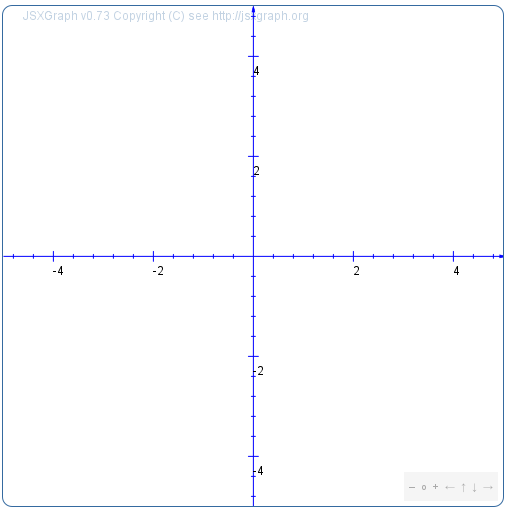
\includegraphics[width=0.4\linewidth]{images/b2.png}}
\caption{The first JSXGraph construction.}\label{fig:1}
\end{figure*}

The complete HTML file then looks like this:
\begin{fullwidth}\begin{lstlisting}[language=HTML]
<html>
<head>
 <link rel="stylesheet" type="text/css" href="jsxgraph.css" />
 <script type="text/javascript" src="prototype.js"></script>
 <script type="text/javascript" src="jsxgraphcore.js"></script>
</head>
<body>
<div id="box" class="jxgbox" style="width:500px; height:500px;"></div>
<script type="text/javascript">
 var board = JXG.JSXGraph.initBoard('box', {boundingbox:[-5,5,5,-5], axis:true});
</script>
</body>
</html>
\end{lstlisting}\end{fullwidth}
Connect JSXGraph with the HTML div tag (usually at the end of the document body) and call 
the method \lstinline|initBoard()| of the global object \lstinline|JXG|

\begin{lstlisting}[language=HTML]
<script type="text/javascript">
 var board = JXG.JSXGraph.initBoard('box', 
            {boundingbox:[-5,5,5,-5], axis:true});
</script>
\end{lstlisting}
The method \lstinline|initBoard()| may have two arguments:
\begin{itemize}
    \item Parameter 1: the \lstinline|id| of the div tag in the HTML page which will contain the JSXGraph construction.
    \item (optional) Parameter 2: additional properties of the board. 
\end{itemize}
The possible optional properties of the board are:

    * originX, originY (in pixel)
    * unitX, unitY (in pixel)
    * zoomX, zoomY
    * Bounding box
    * axis (true/false)
    * grid (true/false)
    * showNavigation (true/false)
    * showCopyright (true/false) 

More than one boards can be initialised simultaneously in one HTML file. 
%%%%%%%%%%%%%%%%%%%%%%%%%%%%%%%%%%%%%%%%%%%%%%%%%%%%%%%%%%%%%%%%%%%%%%%%%%%%%%%%%%%%%%%%%%%%%
\chapter{Creating geometric elements}

The next step is to create geometric elements in the drawing panel which can be 
dragged around.
Through the JavaScript variable \lstinline|board| in the above listing we have access to the drawing panel 
and can place objects there. New geometry elements can be added to the board. 
All elements are added with the method \lstinline|board.createElement()|. One example:
\begin{lstlisting}
board.createElement('point', 
        [1,3], 
        {name:'A', strokecolor:'red'}
        );
\end{lstlisting}
Another example:
\begin{lstlisting}
board.createElement('point', 
        [function(){return s.X();},function(){return t.X()}], 
        {trace:true}
        );
\end{lstlisting}
The parameters of the method \lstinline|board.createElement()| are:
\begin{lstlisting}
board.createElement(elementType, parents, attributes);
\end{lstlisting}
where
\begin{itemize}
    \item \lstinline|elementType| is a string containing the type of the element which is constructed. 
       At the moment, possible types are:
        \begin{itemize}
          \item primitive elements like points, lines, curves
          \item composite elements like bisectors, midpoints 
        \end{itemize}
    \item \lstinline|parents| is an array containing the parameters which define the element. 
    This can be parent elements like two points which define a line. It can also consist of JavaScript functions, numbers, and strings containing \geonext{}\sidenote{see http://geonext.de} syntax. The possible array elements depend on the element type.
    \item \lstinline|attributes| is an optional argument and has to be a JavaScript object. 
    Usually it is given in the form 
    \lstinline|{key1:value1, key2:value2, ...}|, called the ``literal object'' form.
\end{itemize}

\subsection{Construction of a free point}
This example in Figure~\ref{fig:2} shows how to construct a simple, draggable point. 
\begin{figure*}[htb]
\centerline{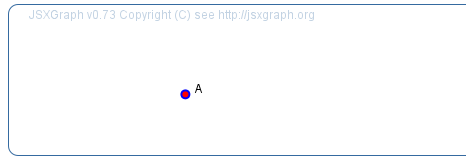
\includegraphics[width=0.4\linewidth]{images/b3.png}}
\caption{The first JSXGraph point.}\label{fig:2}
\end{figure*}
It is produced by the following commands:
\begin{lstlisting}[language=html]
<div id="box" class="jxgbox" 
    style="width:200px; height:200px;"></div>
<script type="text/javascript">
 var board = JXG.JSXGraph.initBoard('box', 
                {boundingbox:[-2,2,2,-2]});
 var p = board.createElement('point',[1,1]);
</script>
\end{lstlisting}

The JavaScript code has to be placed {\sl after} the div element which will contain the construction. From now on, we will only show the JavaScript code. 

\subsection{Attributes of a point}
Several attributes can be given to change the properties of a point, for example a name or the point style. 
\begin{lstlisting}
 var board = JXG.JSXGraph.initBoard('box', 
                {boundingbox:[-2,2,2,-2]});
 var p = board.createElement('point',[1,1],{name:'X',style:5});
\end{lstlisting}
The resulting point in Figure~\ref{fig:3} is now labeled with ``X''.
\begin{figure*}[htb]
\centerline{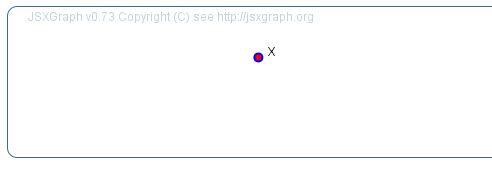
\includegraphics[width=0.4\linewidth]{images/b4.png}}
\caption{The JSXGraph point ``X''.}\label{fig:3}
\end{figure*}

\paragraph{Point styles}
The layout of a point can be influenced by the property \lstinline|type|. It can attain the values $0,1,\ldots,12$. 
Alternatively of these equivalent constants can be used:

\bigskip
\begin{center}
\footnotesize
\begin{tabular}{lll}
\toprule
Constant &    value   & description \\
\midrule
\lstinline|JXG.POINT_STYLE_X_SMALL| &     0  & Small x \\
\lstinline|JXG.POINT_STYLE_X|  & 1&   Medium x \\
\lstinline|JXG.POINT_STYLE_X_BIG|  & 2  & Big x \\
\lstinline|JXG.POINT_STYLE_CIRCLE_TINY|  &   3 &  Tiny circle \\
\lstinline|JXG.POINT_STYLE_CIRCLE_SMALL|  &  4  & Small circle \\
\lstinline|JXG.POINT_STYLE_CIRCLE| & 5 &  Medium circle \\
\lstinline|JXG.POINT_STYLE_CIRCLE_BIG| & 6  & Big circle \\
\lstinline|JXG.POINT_STYLE_SQUARE_SMALL|&   7&   Small square \\
\lstinline|JXG.POINT_STYLE_SQUARE|&  8  & Medium square \\
\lstinline|JXG.POINT_STYLE_SQUARE_BIG|&  9 &  Big square \\
\lstinline|JXG.POINT_STYLE_PLUS_SMALL|&  10 & Small $+$ \\
\lstinline|JXG.POINT_STYLE_PLUS|&   11  &Medium $+$ \\
\lstinline|JXG.POINT_STYLE_PLUS_BIG| &   12  &Big $+$ \\
\bottomrule
\end{tabular}
\end{center}
In the following example we use a for loop to create $13$ points attaining all possible styles. The result can be see in Figure~\ref{fig:4}.
\begin{lstlisting}
var board = JXG.JSXGraph.initBoard('box', 
                {boundingbox:[-2,2,2,-2]});
for (var i=0;i<13;i++) {
  var p = b3.createElement('point',[i,0], 
                {name:'P_{'+i+'}', style:i});
}
\end{lstlisting}
\begin{figure*}[h]
\centerline{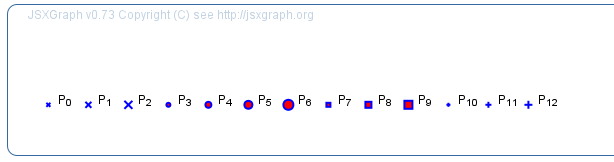
\includegraphics[width=0.4\linewidth]{images/b5.png}}
\caption{All possible point styles.}\label{fig:4}
\end{figure*}
Other attributes of a point are
\bigskip
\begin{center}
\footnotesize
\begin{tabular}{lll}
\toprule
attribute name &    value   & description \\
\midrule
style                   & $0\ldots12$ & see above\\
strokeColor             & color string & \\
strokeWidth             & color string & \\
fillColor               & color string & \\
highlightStrokeColor    & color string & \\
highlightFillColor      & color string & \\
labelColor              & color string & \\
visible                 & \lstinline|true|,\lstinline|false|& point and label are visible\\
fixed                   & \lstinline|true|,\lstinline|false|& dragging possible \\
draft                   & \lstinline|true|,\lstinline|false|&  \\
trace                   & \lstinline|true|,\lstinline|false|& dragging leaves a trace\\
withLabel               & \lstinline|true|,\lstinline|false|& point has a label\\
name                    & string& label text this element\\
id                      & string&  unique id for this element\\
\bottomrule
\end{tabular}
\end{center}
If not given \lstinline|name| and \lstinline|id| are chosen automatically.

All properties beside \lstinline|id| can be changed during the life time of an object \lstinline|el|
using the method \lstinline|el.setProperty|. There are several formats possible.
\begin{lstlisting}
el.setProperty('key1:value1','key2:value2',...);
el.setProperty([key1:value1],[key2:value2],...);
el.setProperty({key1:value1, key2:value2,...});
\end{lstlisting}

\end{document}
